\chapter{Model zur Lösung des CSP-Problems}\label{model}
\section{Implementierung des Min-Conflicts-Embedder}

Die Implementierung des Min-Conflicts-Embedder ist anhand des Aktivitätsdiagramm (Abbildung \ref{fig:minConflictsAkti}) graphisch dargestellt. Zuerst wird die Schleifenvariable der äußeren Schleife mit Null initialisiert und die Methode \textbf{mapTaskRandomly} aufgerufen. In \textbf{mapTaskRandomly} werden alle Tasks einer zufällig gewählten Kachel, die im Programmcode Unit genannt wird, zugewiesen. Es werden dabei Verletzungen der Constraints ignoriert. Anschließend wird der inneren Schleifenvariable k dem Wert Null zugewiesen und die Funktion \textbf{findRandomConflictingTask} aufgerufen. Diese Funktion wählt einen Task aus der Menge C der Tasks aus, die mindestens einen Constraint verletzen. Falls es keinen Task gibt (conflictingTask==null) und somit die Menge C leer ist, wurde eine Lösung gefunden (\textbf{success}). Ansonsten wird überprüft, ob die maximale Anzahl an Schleifendurchgängen (kMax) erreicht wurde. Wenn dies nicht der Fall ist, ruft das Programm die Funktion \textbf{minConflicts} auf. \textbf{minConflicts} bekommt als Parameter den conflictingTask übergeben und versucht für ihn eine geeignete Kachel zu finden, die zu keiner Verletzung eine Bindungs- bzw Routingbedingung führt. Falls es eine derartige Kachel nicht gibt, wird schrittweise der MaxHopConstraint gelockert. Das heißt, dass die Manhattendistanz schrittweise um eins erhöht wird, bis der Algorithmus eine geeignete Kachel gefunden hat. Ist dies der Fall, wird k inkrementiert und die Funktion \textbf{findRandomConflictingTask} wiederum aufgerufen. \\
Hat k den Wert kMax erreicht, so ist der Durchgang beendet und alle Tasks werden ihrer Kachel entzogen (\textbf{unmapTasks}). Die Funktion \textbf{mapTaskRandomly} wird aufgerufen und ein neuer Durchgang beginnt. Falls nach jMax Durchgängen noch keine Lösung gefunden wurde, beendet sich das Programm (\textbf{fail}).

\begin{figure}[H]\centering
  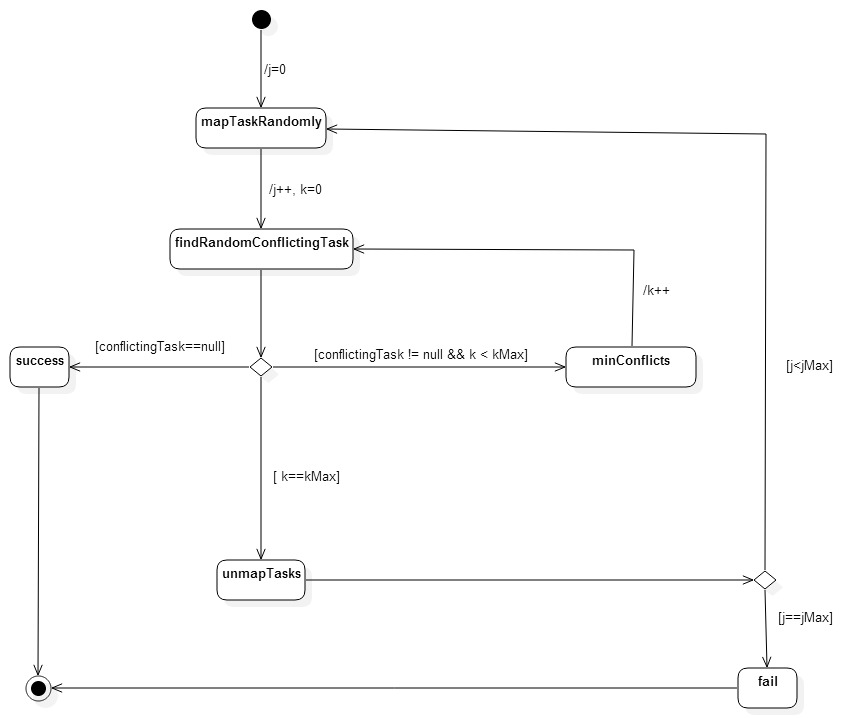
\includegraphics[width = 150mm]{bilder/minAkti.jpg}
  \caption{Das Aktivitätsdiagramm zur Min-Conflicts-Implementierung}\label{fig:minConflictsAkti}
\end{figure}
\section{Klassendiagramm zum Lösen der Bindungs- und Routinganforderungen}


\subsection{Bindungsanforderungen}

Die Abbildung \ref{fig:klBind} zeigt das Klassendiagramm zum Lösen von Bindungsanforderungen. Die Klasse Task speichert in einer Liste alle Bindungsanforderungen (engl. TaskConstraints) ab und stellt folgende Funktionen zur Verfügung:

\begin{itemize}
\item \textit{addTaskConstraint}\\
fügt ein Objekt einer abgeleiteten Klasse von TaskConstraints der Liste hinzu. 
\item \textit{removeTaskConstraint}\\
löscht ein Objekt einer abgeleiteten Klasse von TaskConstraints aus der Liste
\item \textit{taskConstraintsAreSatisfied}\\
ruft für alle Objekte in der Liste die Funktion isSatisfied aus der Klasse TaskConstraints auf. isSatisfied überprüft, ob die jeweilige Bindungsanforderung erfüllt ist. Die Funktion gibt True zurück, wenn alle Bindungsanforderungen erfüllt sind.%Es wird True zurückgegeben, wenn für alle Objektaufrufe
\item numberOfFailingConstraints\\
gibt die Anzahl der fehlgeschlagenen Bindungsanforderungen zurück, wenn man dem Task eine Unit u zuweist. 
\item mapConstraints\\
weist dem Task eine Unit zu. Alle Objekte, die sich in der Liste befinden, rufen die Methode map auf.
\item unmapConstraints\\
entzieht dem Task die Unit. Alle Objekte, die sich in der Liste befinden, rufen die Methode unmap auf.
\end{itemize}

Um von der abstrakten Klasse TaskConstraints zu erben, müssen diese abstrakten Methoden implementiert werden:\\
\begin{itemize}
\item isFeasible\\
überprüft, ob bei Einbetten des Tasks zur Unit u die durch das Objekt repräsentierte Anforderungen erfüllt werden würde. Hierzu wird die Methode check mit der Objektvariable der zugehörigen Instanz der Klasse UnitAttributes aufgerufen. \todo{Umformulierung}
\item isSatisfied\\
überprüft, ob der eingebettete Task, die durch das Objekt repräsentierte Anforderung, erfüllt. Dazu wird die Methode check der zugerhöirigen UnitAttributes-Klasse mit dem Übergabewert null aufgerufen. 
\item map \\
ruft von der zugehörigen UnitAttributes Unterklasse die Methode update auf. Der Parameterwert ist die eigene Objektvariable
\item unmap\\
ruft von der zugehörigen UnitAttributes Unterklasse die Methode update auf. Der Parameterwert ist der negierte Wert der eigenen Objektvariable
\end{itemize}

Die Klasse Unit repräsentiert eine Kachel dem Network-on-Chip. Jede Instanz ist durch die Positionsangabe (x,y) eindeutig identifizierbar. Eine Instanz erhält Objekte der abgeleiteten Unterklassen von der abstrakten Klasse UnitAttributes. Die Klasse Unit befinden sich folgende Methoden:
\begin{itemize}
\item addUnitAttriubte\\
fügt der Liste eine Objekt einer Unterklasse von UnitAttributes hinzu
\item removeUnitAttriubte\\
löscht ein Objekt einer Unterklasse von UnitAttributes aus der Liste
\end{itemize}

Die Kindklassen von UnitAttributes müssen die zwei Methoden check und update implementieren. Jede Kindklasse von UnitAttributes wird dabei von genau einer Kindklasse von TaskConstraints verwendet.

\begin{itemize}
\item check\\
überprüft, ob es möglich ist, dass Attribut zu aktualisieren.
\item update \\
aktualisiert die Objektvariable des Attributs.
\end{itemize}

%\todo{TyeAttribute wird nichts upgedated}

TypeAttribute ist hierbei ein Spezialfall. Hier kann die Objektvariable nicht, wie z. B. bei UnitWorkloadAttribute, aktualisiert werden, da sich der Ressourcentyp  nicht während der Laufzeit verändern lassen kann. So macht in diesem Fall die Funktion update das gleiche wie check. Es überprüft nur, ob der gewünschte Ressourcentyp vorliegt.

\begin{figure}[H]\centering
  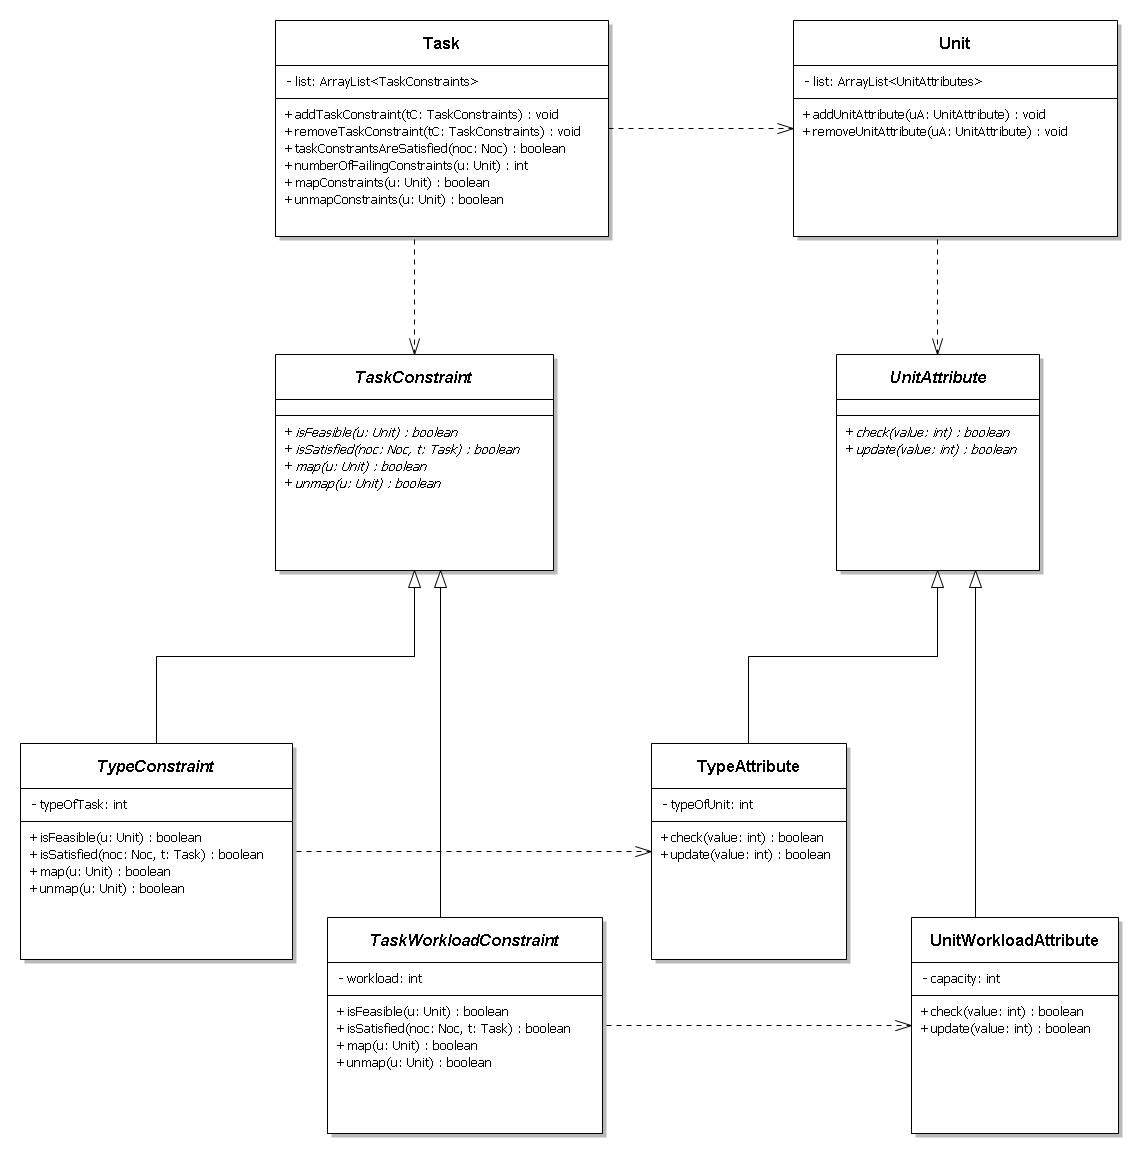
\includegraphics[width = 150mm]{bilder/task-unit.jpg}
  \caption{Klassendiagramm zum Lösen von Bindungsanforderungen}\label{fig:klBind}
\end{figure}

\subsection{Routinganforderungen}

Das Klassendiagramm zum Lösen von Routinganforderungen (siehe Abbildung \ref{fig:klRoute}) ist dem von Bindungsanforderungen sehr ähnlich. So sind die Methoden und deren Funktionalitäten gleich. Der größte Unterschied zu den Bindungsanforderungen besteht darin, dass nicht wie bei den Bindungsanforderungen die Attribute von nur einer Kachel (Unit) überprüft bzw. aktualisiert werden. Bei den Routinganforderungen werden die Attribute von mehreren Links, die zuvor mithilfe eines Routingalgorithmuses gefunden wurden, nachgeprüft oder erneuert.
\begin{figure}[H]\centering
  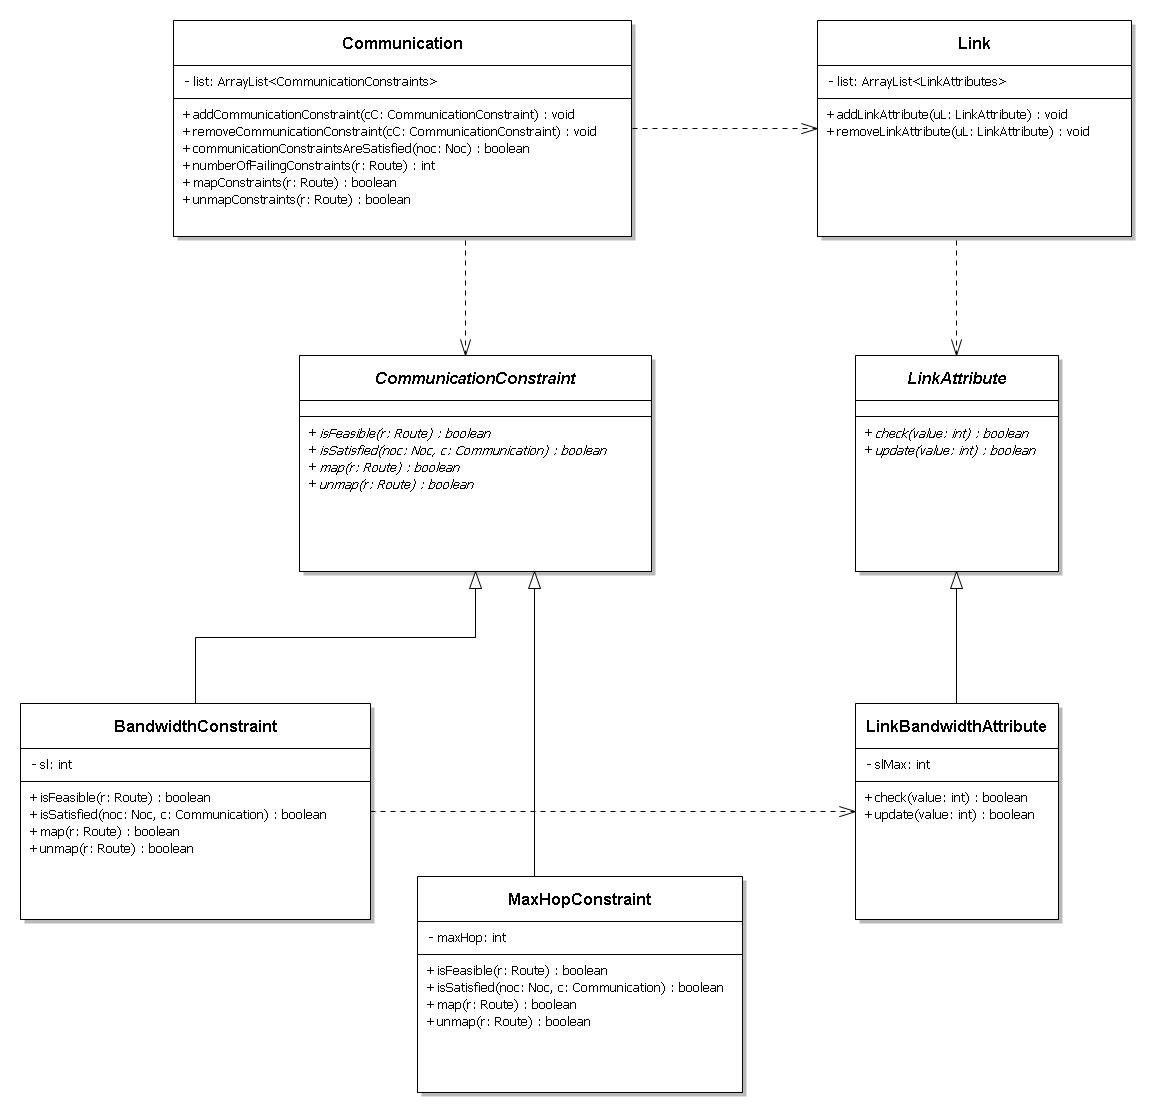
\includegraphics[width = 150mm]{bilder/communication-link.jpg}
  \caption{Klassendiagramm zum Lösen von Routinganforderungen}\label{fig:klRoute}
\end{figure}